The Radix sort is another example of a sorting algorithm having both a serial and an parallel implementation. The Radix sort can be considered brute force, and is a non-comparison algorithm. The idea behind the radix sort is to sort each elements by its elements bits. The way the radix sort works can be divided into three steps as seen in \cref{tab:radix}.

\begin{center}
	\fbox{
		\begin{tabular}{p{40pt} p{220pt}}
			\textbf{Step 1} & Start with LSB \\
			\textbf{Step 2} & Split input into 2 sets based on bit values, otherwise preserve order \\
			\textbf{Step 3} & Move to next MSB, repeat
		\end{tabular}
	}
	\captionof{table}{Steps of Radix sort}
	\label{tab:radix}
\end{center} 

An example of the radix sort with the steps form \cref{tab:radix} is seen in \cref{fig:sort_radix}.

\begin{figure}[ht]
	\centering
	\fbox{
		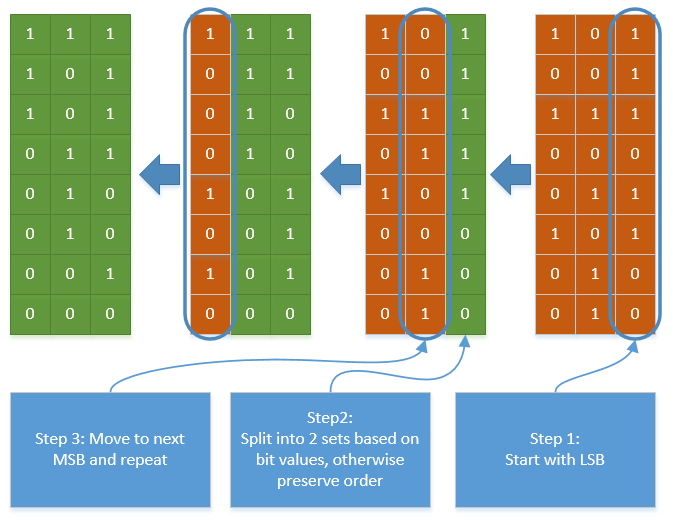
\includegraphics[width=0.7\textwidth]{figs/algorithm/sort_radix.png}}
	\caption{Radix sort}
	\label{fig:sort_radix}
\end{figure}  

The Radix sort have a work complexity of $\mathcal{O}(kn)$ where k is the number og bits, and a step complexity of $\mathcal{O}(k)$. The radix sort is therefore highly depended on the number of bits in the numbers to sort. The radix will also often have a better work and step complexity, when compared with other sorting algorithms. The radix sort is a good example of an algorithm that is not very efficient in serial, but rather efficient in parallel, because of the high parallelization. The implementation of the radix sort is explained in the \cref{sec:exercise4}.   
